\documentclass[12pt]{article}

\usepackage{amsmath}
\usepackage{amssymb}
\usepackage{calc}
\usepackage{units}
\usepackage{graphicx}
\usepackage[pdftex]{hyperref}
\usepackage{subfig}
\usepackage[margin=1in]{geometry}
\usepackage{listings}
\usepackage[numbers,sort&compress]{natbib}
\usepackage{bm}
\usepackage{paralist}
\usepackage[draft]{fixme}

\hypersetup{
  breaklinks=true,
  pdftitle={Measuring Electric Phenomena: the Ammeter and Voltmeter},
  pdfauthor={Kevin R. Lynch}, 
  pdfsubject={Phyiscs, Electricity and magnetism},
  pdfkeywords={ammeter, voltmeter, multimeter},
  pdflang={en-US},
}

\title{Measuring Electric Phenomena:\\the Ammeter and Voltmeter}
\author{}
%Kevin R. Lynch
%\date{2015-01-28}
\date{}

\begin{document}

\maketitle

\section{Objectives}
\label{sec:objectives}

\begin{enumerate}
\item To understand the use and operation of the Ammeter and
  Voltmeter in a simple direct current circuit, and
\item To verify Ohm's Law for the resistor.
\end{enumerate}

\section{Introduction}
\label{sec:introduction}

The German physicist, Georg Ohm, was the first to explore the
relationship between the current \textit{through} an object compared
to the voltage applied \textit{across} that object.  He published his
results, \textit{Die galvanische Kette, mathematisch
  bearbeitet}\footnote{The galvanic circuit investigated
  mathematically}, in 1827.  His results were not immediately
accepted, because his methods were so revolutionary, and challenged
the accepted requirements of scientific reasoning of his day; science
is a human endeavor, and this result has a fascinating backstory that
I urge you to investigate.

To investigate the properties of voltage and current, and the
relationship between the two, we need tools and equipment to do it.
We measure voltage with the \textit{voltmeter}, and current with the
ampmeter or \textit{ammeter}.  In a later lab, you will study the
detailed properties of ideal meters, and contrast them with the real
meters that we can actually build.  In this lab, however, you will
learn the proper use of these devices while investigating Ohm's Law.

\section{Theory}
\label{sec:theory}

Ohm showed that a \textit{steady} current was caused by a
\textit{constant} voltage, that were directly proportional to each
other, and that they scaled with the length of the \textit{resistive}
element through which the current flowed.  Today, we express this
relationship mathematically as $V/I \propto 1$, where $V$ is the
voltage (measured in the SI system in \textit{volts}, $V$) and $I$ is
the current (measured in \textit{amperes}, $A$).  We give the
\textit{constant of proportionality} the name \textit{resistance}, and
the symbol $R$
\begin{gather*}
  R = \frac{V}{I} \ ,
\end{gather*}
Resistance is measured in \textit{ohms}, with the symbol $\Omega$.

Ohm's Law is - despite its name - \textit{not} a law of nature;
instead, it is an empirical relationship for many materials under many
reasonable conditions.  In this lab, the resistance $R$ will be
constant for a given object.  In other labs, we will investigate the
limits of this relationship: under what conditions does it hold true,
when does it fail, and how can we understand these properties as the
results of microscopic physics.

Let's now introduce the voltmeter and the ammeter.  A voltmeter is
designed to measure the voltage \textit{across} a portion of a
circuit, that is, between \textit{two points} in an electrical system.
An ammeter is designed to measure the current \textit{passing through}
a \textit{single point} in the circuit.  The voltmeter stays
\textit{outside} the circuit, while the ammeter must be inserted
\textit{into} the circuit.  While these devices have distinct
properties and uses, the ammeter and voltmeter are such a basic part
of the scientific measurement toolkit that the are usually found
integrated into a single device called the \textit{multimeter}.  There
are many kinds of multimeters: desktop or handheld, analog or digital,
manual or autoranging, low and high voltage, etc.  Beware, however!
Switching a multimeter from ammeter to voltmeter mode usually requires
the inputs to be rewired; failing to do so can result in blown fuse,
or damaging the device.  And finally, for safety reasons, never use a
multimeter for measurements in high voltage circuits, unless you have
been specifically trained for that task!  We won't be exposing you to
such risks in this course.

In order to talk in more detail about these devices, we need a
language describe the connections between them in a particular
\textit{electrical circuit} - the circuit diagram, or schematic.
Schematics are a kind map: they make explicit the wired connections
between electrical devices in a circuit.  They are, however, not a
photograph, and are usually not to scale - much like the New York City
subway map, they don't show everything that's going on, only the
critical details.  The connections between devices in a diagram do not
indicate literal wires, but only the required relationships (ie
``topological connections'') between the devices; for practical
reasons, there may be multiple ways to connect the devices, requiring
more or fewer actual wire than shown in the diagram.  There may also
be multiple physical realizations, or \textit{layouts}, of a given
schematic, and there may be multiple equivalent schematics for a given
layout.

\begin{table}
  \centering
  \begin{tabular}{|l|c|}\hline
    Resistor & 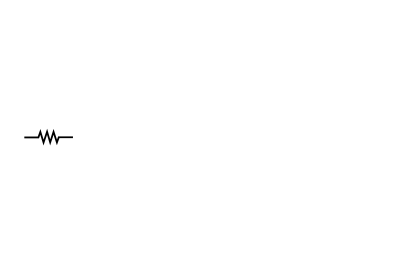
\includegraphics[width=1in]{figures/resistor}\\ \hline
    Voltmeter & 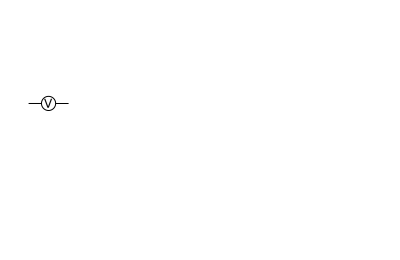
\includegraphics[width=1in]{figures/voltmeter}\\ \hline
    Ammeter & 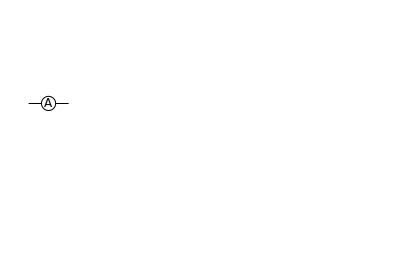
\includegraphics[width=1in]{figures/ammeter} \\ \hline
    DC Voltage source & 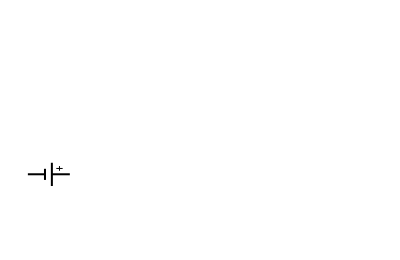
\includegraphics[width=1in]{figures/dc_supply}\\ \hline
  \end{tabular}
  \caption{The various schematic elements used in this lab.}
  \label{tab:schematic}
\end{table}
The language of circuit schematics is highly evolved, and there are
\textit{de facto} standard representations of typical devices.
Table~\ref{tab:schematic} contains the common symbols used in this
lab.

When learning to build or ``wire'' a circuit from a schematic, it is
usually best to arrange your physical devices (resistors, power
supplies, meters, etc.) in the same orientation as the devices on the
schematic.  Then, follow the ``map'' given by the schematic: pick one
terminal on the first device, and locate all the terminals on other
devices that are connected to that terminal on the schematic.  Using
one or more wires, reproduce those schematic connections in the
physical world.  Repeat until you have ``visited'' all terminals on
the schematic.  Note that not all terminals may be labeled identically
on the schematic and on the physical devices: they may be labeled the
same, differently, or perhaps not labeled at all!  You will need to
use your judgment, ask questions of your instructor, or simply try an
experiment to figure things out on your own.

\section{Procedures}
\label{sec:procedures}

\begin{figure}
  \centering
  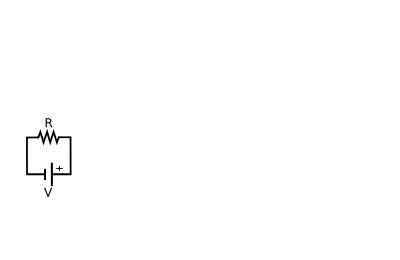
\includegraphics[width=\textwidth/5]{figures/simplest}
  \caption{The simplest direct current circuit.}
  \label{fig:simple}
\end{figure}
\begin{figure}
  \centering
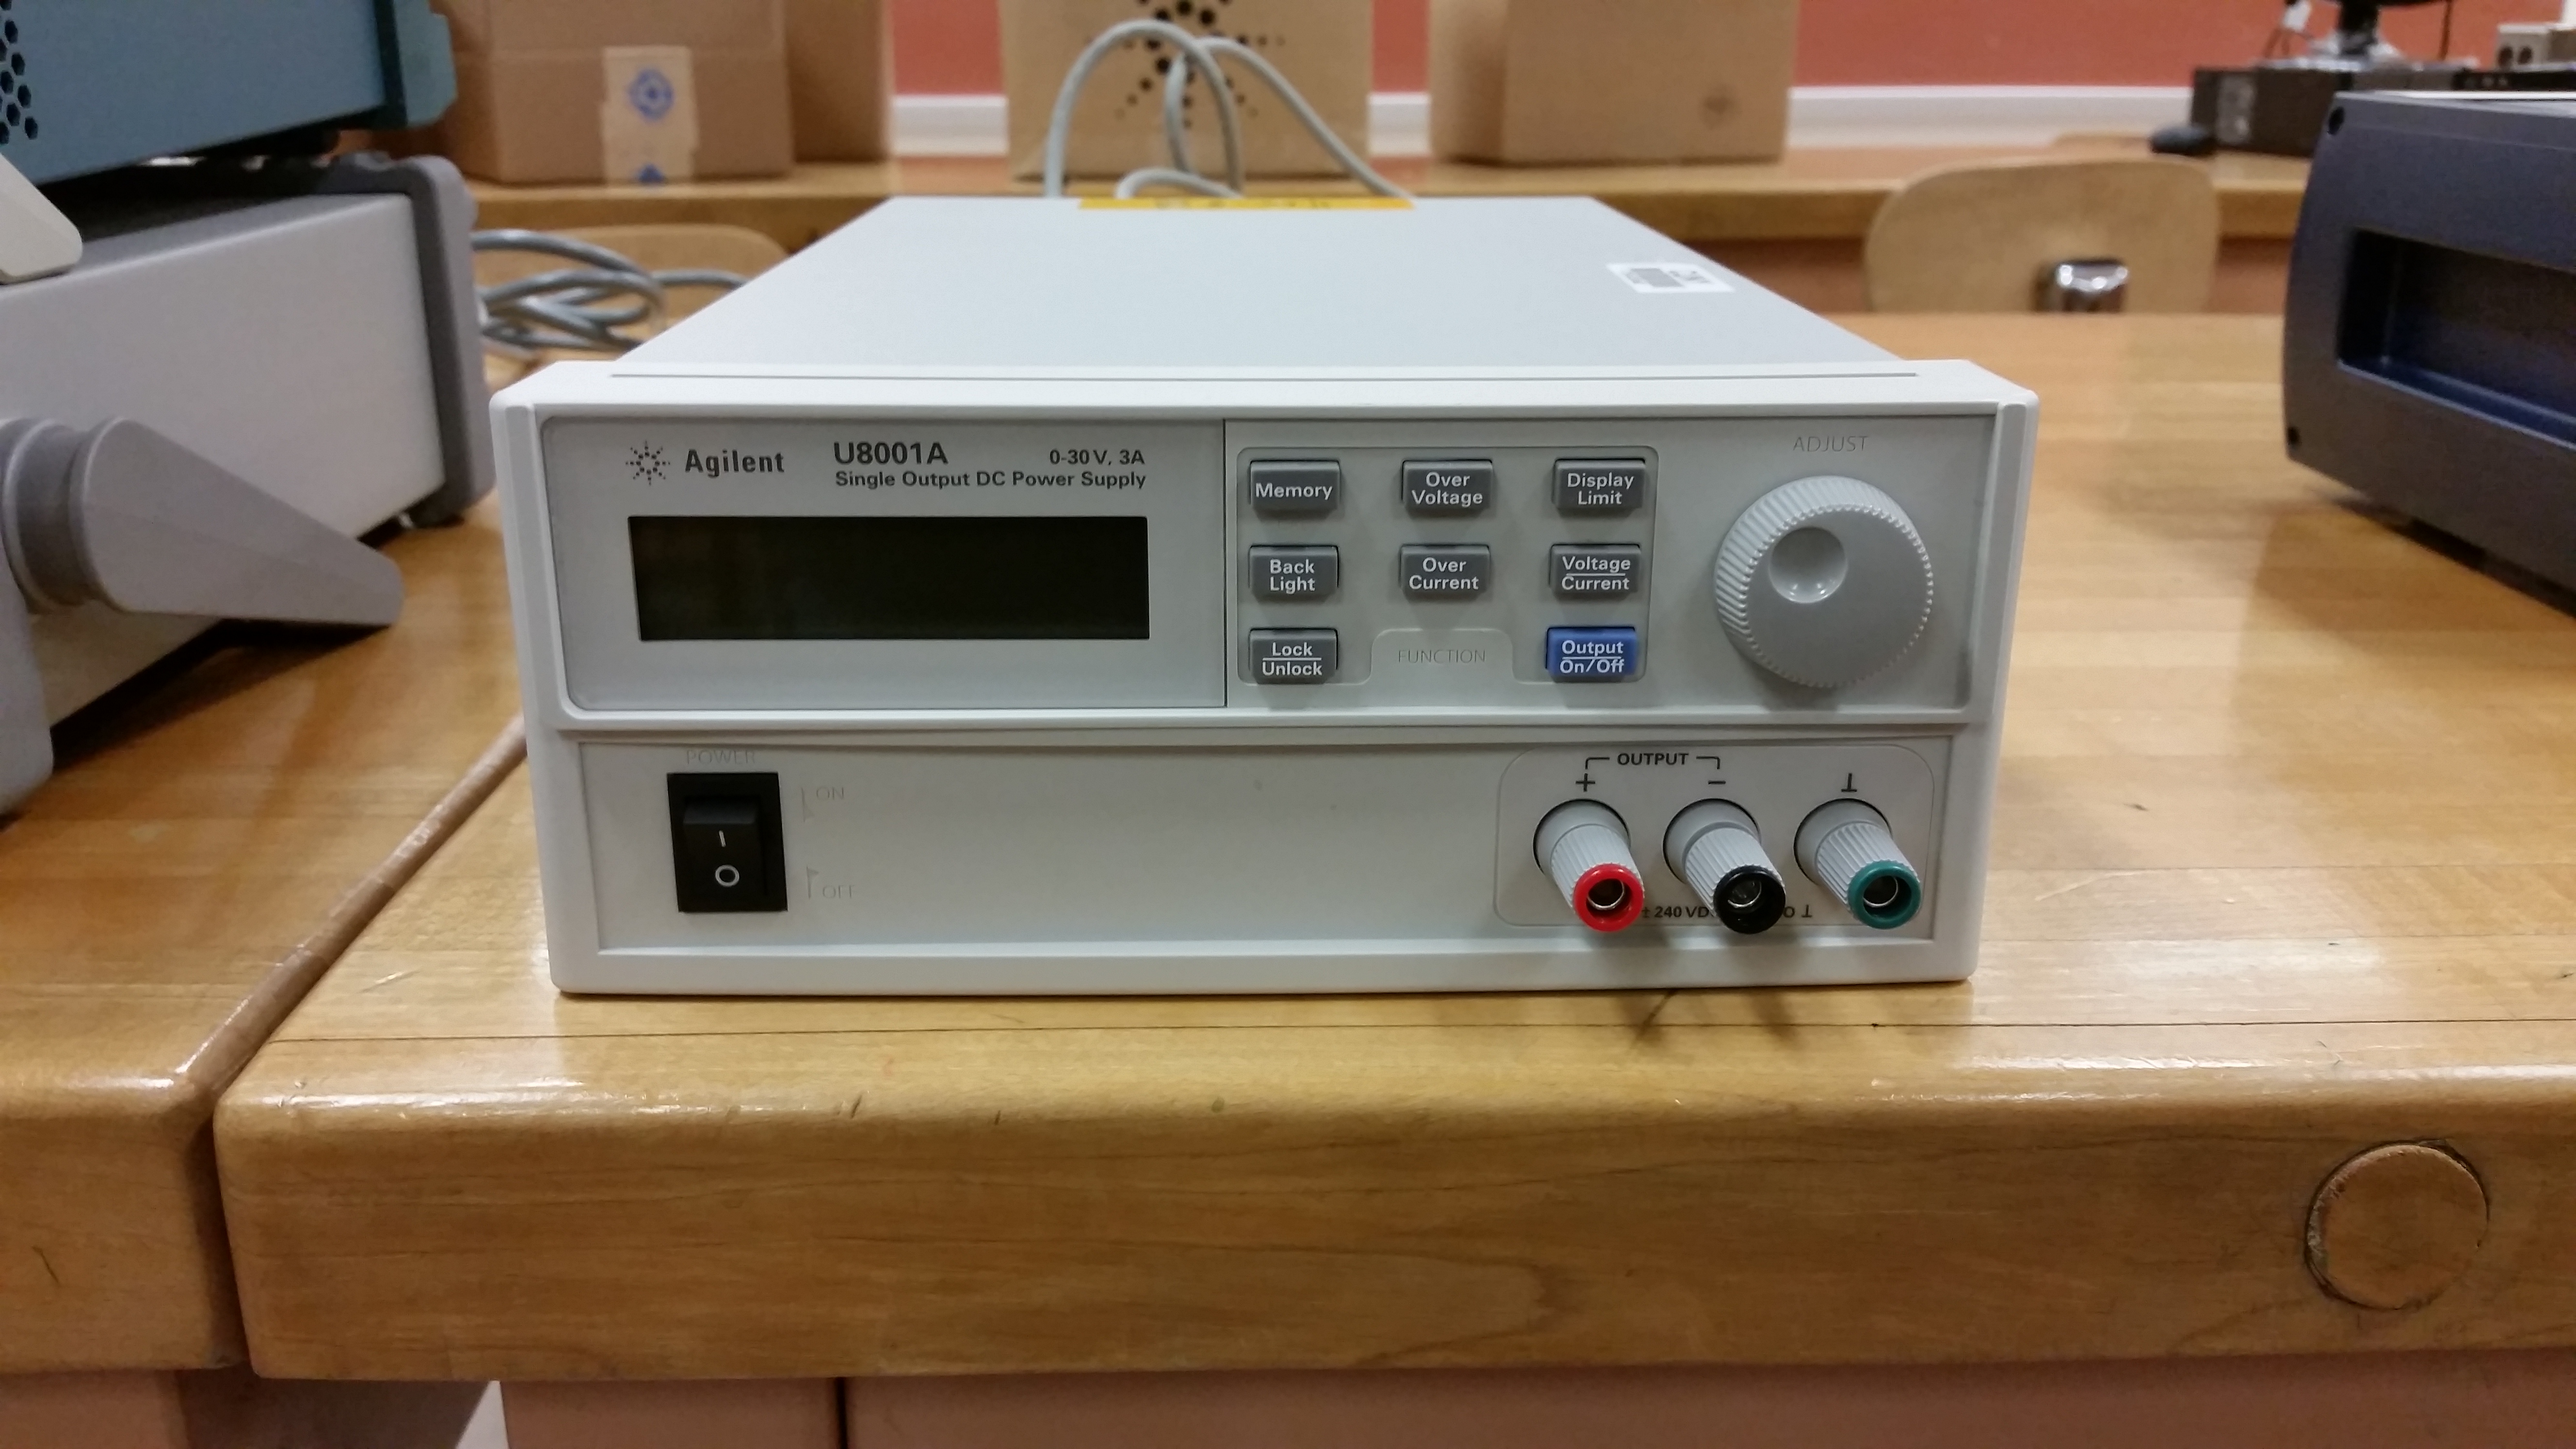
\includegraphics[width=\textwidth/2]{figures/agilent_u8001a}
  \caption{The direct current power supply.}
  \label{fig:dcps}
\end{figure}
\begin{figure}
  \centering
    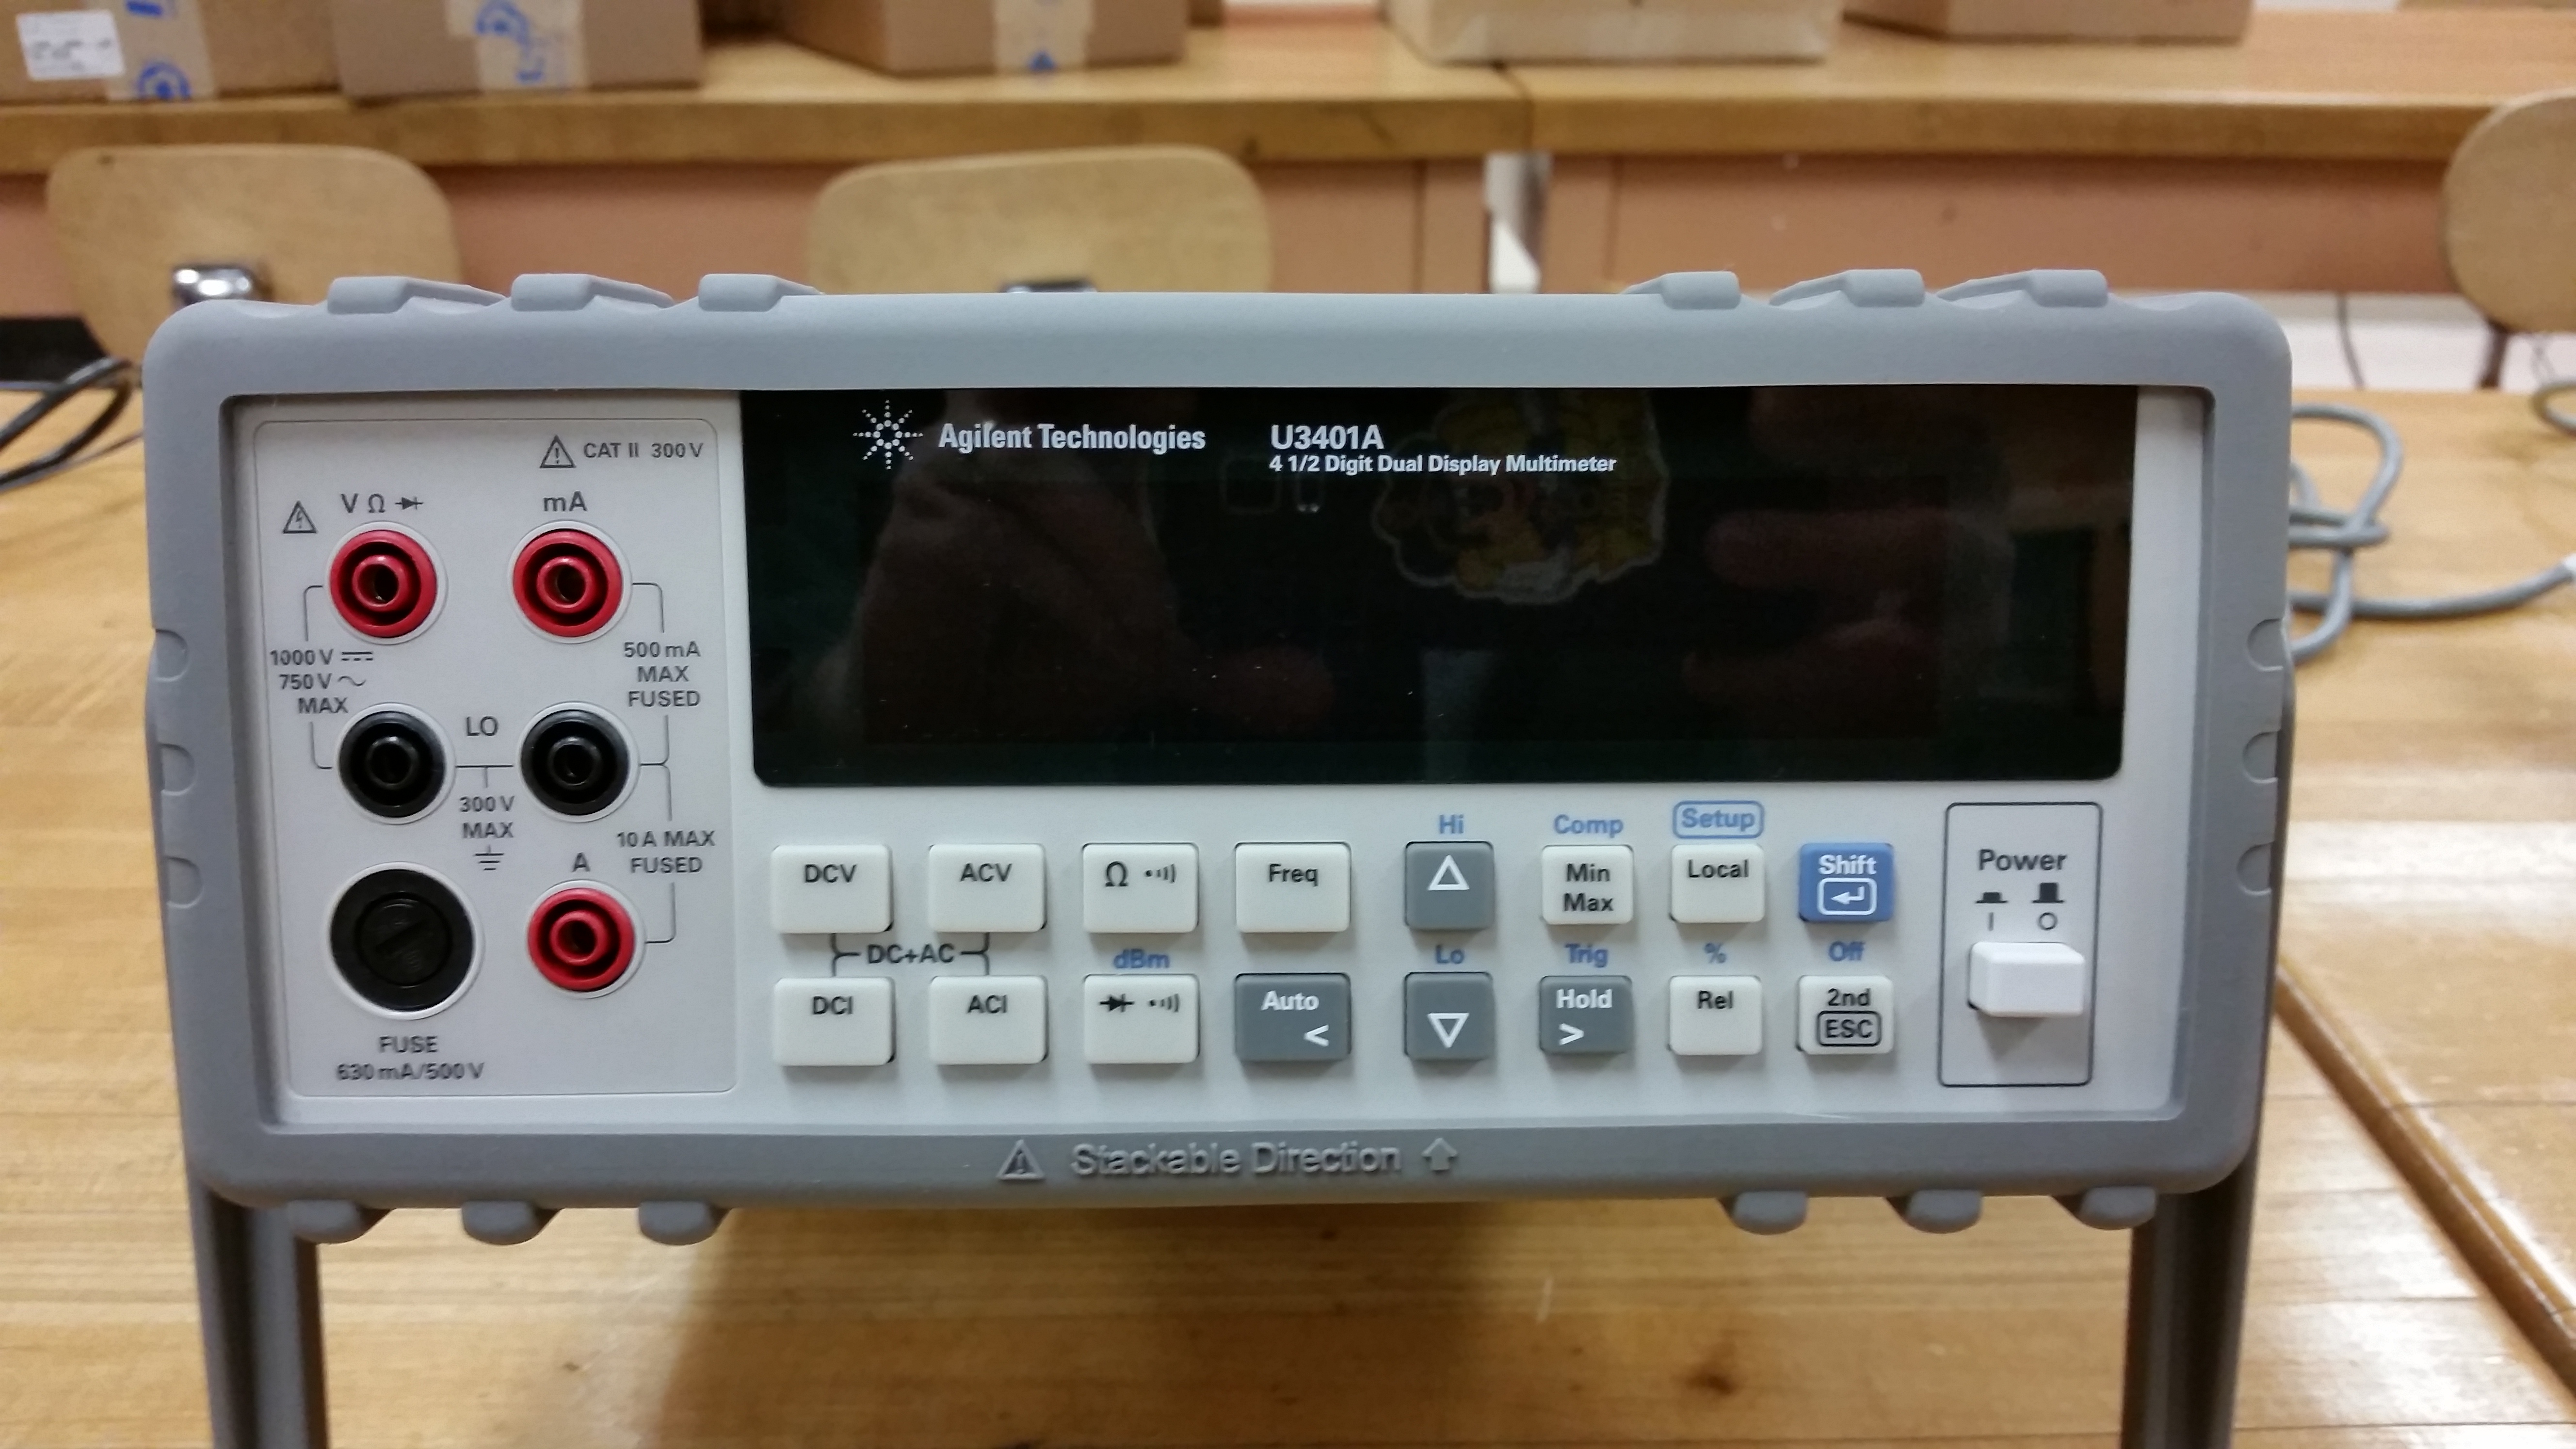
\includegraphics[width=2\textwidth/3]{figures/agilent_u3401a}
  \caption{The multimeter.}
  \label{fig:multimeter}
\end{figure}

In this lab, we will investigate the relationship between current and
voltage in the simplest possible circuit, consisting of a direct
current voltage source and a single resistance
(Figure~\ref{fig:simple}).  You should receive a power supply, two
digital multimeters, and two decade resistance boxes.  The wires you
need are located on a rack in the back of the lab.
\begin{enumerate}
\item First, you have to prepare the power supply, which is the
  \textit{voltage source} for the experiment.  Before connecting the
  anything to the front terminals of the supply, plug it in and turn
  it on.  The outputs will start disabled.  Press the blue
  \textit{Output on/off} button; the display should now show a demand
  voltage and current.  To change the output voltage, you must first
  press the \textit{Voltage/Current} button until the \textit{V}
  annunciator on the display is flashing; now, turn the knob.  Notice
  that the voltage changes.  If you wait long enough, the \textit{V}
  annunciator on the display will stop flashing; turning the knob at
  this point will result in no change to the voltage (Try it!).  This
  is a feature, not a bug \ldots it prevents you from accidentally
  ruining your experiment by turning the knob and unintentionally
  changing the voltage.  Once you are confident you understand how to
  adjust the voltage, set the voltage to zero.
\item Now, construct the circuit shown in Figure~\ref{fig:simple}.
  For the resistor, use one of the two decade resistor boxes; set this
  to something between $\unit[100]{\Omega}$ and $\unit[300]{\Omega}$.
\item Next, configure your first multimeter as a voltmeter.  Plug in
  and turn on the multimeter.  Connect your test leads to the black
  \texttt{LO} and red \texttt{V} inputs, and select the \texttt{DCV}
  (Direct Current Voltage) Function; see Figure~\ref{fig:multimeter}.
\item 
  \begin{figure}
    \centering
    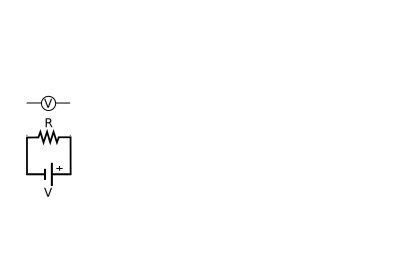
\includegraphics[width=\textwidth/5]{figures/simplest_with_voltmeter}
    \caption{The simplest direct current circuit, with voltmeter installed.}
    \label{fig:simplest_with_voltmeter}
  \end{figure}
  We'll now get a feel for how the meter works.  First, connect the
  test leads to opposite ends of the resistor - that is,
  \textit{across}) the resistor
  (Figure~\ref{fig:simplest_with_voltmeter}).
  
  Now, raise the voltage on the power supply to something like
  \unit[10]{V}; If you have connected the circuit and meter correctly,
  the voltage displayed by the multimeter should roughly match that on
  the supply.  If not, you did something wrong and should ``debug''
  your connections to make sure they are correct.  What happens when
  you swap the leads connected to the resistor?  Why?

  Again, turn the voltage down to zero before proceeding; unless our
  instructions say otherwise, you should always do this before
  changing the configuration of a circuit.
\item 
  \begin{figure}
    \centering
    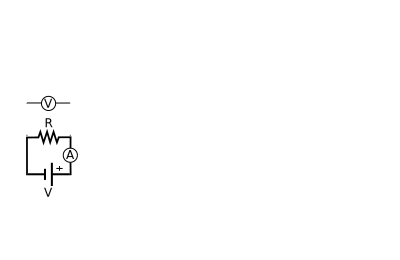
\includegraphics[width=\textwidth/5]{figures/simplest_with_ammeter}
    \caption{The direct current circuit with ammeter inserted.}
    \label{fig:simplest_with_ammeter}
  \end{figure}
  Next, configure the second multimeter as an ammeter: connect your
  test leads to the \texttt{LO} and \texttt{mA} inputs, and select the
  \texttt{DCI} (Direct Current) Function; see
  Figure~\ref{fig:multimeter}.  You measure current \textit{through} a
  device, which means you must insert the meter \textit{into} the
  circuit: you must ``cut'' the circuit, and ``splice'' the meter into
  the ``hole''.  In this case, you should insert the meter between the
  output of the power supply and the resistor.  Make sure the
  voltmeter is still connected across the resistor.  At this point,
  you should have recreated the circuit in
  Figure~\ref{fig:simplest_with_ammeter}.  Again, slowly raise the
  voltage output, and observe the changes in the voltage and current
  values as measured on the respective meters.
\item We are ready to repeat Ohm's measurements!  Vary the voltage in
  small steps (say, ten steps from \unit[0]{V} to \unit[10]{V}), and
  record both the voltage and the corresponding current.  Don't forget
  the units!  Quickly plot your data, $I$ vs $V$: if Ohm was right,
  this should be linear.  Is it?  What is the slope?  How is this
  related to $R$?  You will do this again more carefully in your
  Post-Lab exercises, but it's always a good idea to make ``quick and
  dirty'' plots while taking data to help get a feel for what the data
  may be telling you.  Repeat the measurements; are your results
  consistent?  Select a different resistance value, and repeat your
  measurements.
\item Next, we will use the multimeter in \texttt{Resistance} mode to
  confirm our results.  In this mode, the multimeter performs the same
  experiment we just did in large: it applies a known voltage,
  measures the demand current, and deduces the resistance from these
  two values.  Completely disconnect the circuit.  Connect test leads
  to the \texttt{LO} and \texttt{$\Omega$} inputs, select the
  \texttt{$\Omega$} Function.  Connect the leads to opposite sides of
  the resistor, and record the value.  Does the value you measured
  with the above procedure agree with the value the meter measures
  directly?  With the value you selected on the resistance box?
\item Imagine now that you are the power supply.  When you look out
  from your terminals, all you see is one wire heading out to the
  left, and one wire heading out to the right; you can't actually tell
  what's connected to the wires!  All you can do is measure the
  resistance of the circuit that you are ``driving''.\footnote{We'll
    have a lot more to say about this point of view later in the
    semester, when we talk about not only resistors, but capacitors,
    inductors, diodes, etc.}  In other words, to a DC power supply,
  the whole collection of devices connected to the terminals looks
  like a single resistor; you must be able to predict the effective
  resistance that a collection of devices in a circuit presents to the
  power supply.  In particular, realize that an ammeter or voltmeter
  look \textit{just like any other resistor} to the power supply!  It
  should be obvious that we want to design these meters so that they
  have a minimal impact on the circuit: you don't want to change the
  behavior of the circuit when you connect the meter!  This implies
  different requirements on an ammeter and a voltmeter.  Let's explore
  what happens when you connect multiple resistors in circuit in two
  different ways.  We'll study this in much more detail in a later
  lab; here, we'll explore the implications for the design of the
  meters. 
  \begin{enumerate}
  \item \label{item:identical}
    \begin{figure}
      \centering
      \subfloat[][The series combination.]{
        \label{fig:resistances:series}
        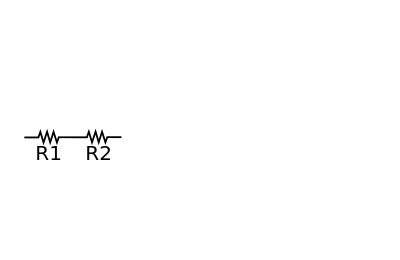
\includegraphics[scale=2.5]{figures/series}
      }\qquad \subfloat[][The parallel combination.]{
        \label{fig:resistances:parallel}
        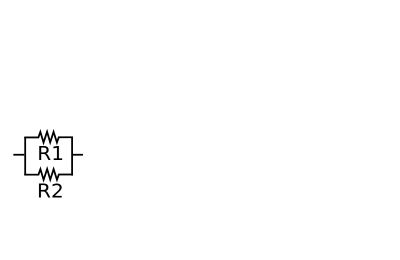
\includegraphics[scale=2.5]{figures/parallel}
      }
      \caption{Series and parallel resistance combinations.}
      \label{fig:resistances}
    \end{figure}
    Configure one of your multimeters to measure resistance.  Set
    \textit{both} of your decade resistance boxes to the same value;
    measure and record both values.  Are they identical?  Why or why
    not?
  \item \label{item:series} Next, wire the circuit shown in
    Figure~\ref{fig:resistances:series}.  This is known as the
    \textit{series} combination of circuit elements: the tail of the
    first element is connected to the head of the second element.
    Measure the resistance of this combination.  How does it compare
    to the individual resistances?  Double one of the resistances, and
    perform the measurement again.  How does it compare?
  \item \label{item:parallel} Reset both resistors to the same value,
    and wire the circuit shown in
    Figure~\ref{fig:resistances:parallel}.  This is the
    \textit{parallel} combination: the heads and tails of the
    resistors are tied together.  Measure the resistance.  How does it
    compare to the individual resistances?  Double one of the
    resistances, and measure again.  How does it compare this time?
  \item You always connect a voltmeter \textit{in parallel} with the
    element you are measuring across, and you connect an ammeter
    \textit{in series} with the element you are measuring the current
    through.  Ideally, what would the resistance of the ammeter be so
    as not to change the behavior of the circuit?  The voltmeter?
    Why? 
  \end{enumerate}
\end{enumerate}

Make sure you clean up your work space, and return every item to the
condition and location you originally found them in!

\newpage

\section*{Pre-Lab Exercises}

Answer these questions as instructed on Blackboard; make sure to
submit them before your lab session!

\begin{enumerate}
\item What do you use a voltmeter for?
\item How about an ammeter?
\item If you double the resistance in a circuit while keeping the
  current unchanged, what happens to the voltage?  What if, instead,
  you keep the voltage unchanged?
\item Sketch the relationship between voltage and current implied by
  Ohm's Law.
\end{enumerate}

\newpage

\section*{Post-Lab Exercises}

\begin{enumerate}
\item Prepare a neatly organized tabulation of your recorded data.
  Make sure to label your data, and include units where appropriate.  
\item Plot all of your data sets on a single graph, preferably by
  computer.  If Ohm was right, this should be linear.  Is it?  Does
  your data support or refute Ohm's Law?  Why or why not?  How do you
  determine the value of the resistance from your plot?  Does it agree
  with the values you measured directly with the multimeter?  Why or
  why not?
\item In Step~\ref{item:identical} of the procedure, you separately
  measure the values of two ``identical'' resistors.  Were they
  identical?  Why or why not?
\item When you combine resistors in series and parallel (as you did in
  Steps~\ref{item:series} and~\ref{item:parallel} of the procedure),
  the resistance of the combination can be predicted if you know the
  individual resistances.  Can you make an educated guess as to the
  correct formulae for these combinations?
\item Ideally, what would the resistance of the ammeter be so as not
  to change the behavior of the circuit?  The voltmeter?  Why?
\item Imagine you have a circuit consisting of two resistors and one
  power supply.  How many different ways are there to connect these
  elements into a circuit?  Draw schematics for all the possible
  inequivalent circuits.  Make sure to label the components.  For one
  of these circuits, draw a new diagram showing how you would connect
  a multimeter to measure the voltage across the power supply, and
  another to show how you would measure the voltage across one of the
  resistors.
\item Discuss briefly whether you have met the objectives of the lab
  exercises.  
\end{enumerate}

\end{document}

%%% Local Variables: 
%%% mode: latex
%%% TeX-master: t
%%% End: 
